\documentclass[12pt,a4paper,article]{article}

\usepackage[a4paper, mag=1000, left=2.5cm, right=1cm, top=2cm, bottom=2cm, headsep=0.7cm, footskip=1cm]{geometry}
\usepackage[utf8]{inputenc}
\usepackage[english,russian]{babel}
\usepackage{indentfirst}
\usepackage[dvipsnames]{xcolor}
\usepackage[colorlinks]{hyperref}
\usepackage{listings} 
\usepackage{fancyhdr}
\usepackage{caption}
\usepackage{graphicx}
\hypersetup{
	colorlinks = true,
	linkcolor  = black
}

\usepackage{titlesec}
\titleformat{\chapter}
{\Large\bfseries} % format
{}                % label
{0pt}             % sep
{\huge}           % before-code


\DeclareCaptionFont{white}{\color{white}} 

% Listing description
\usepackage{listings} 
\DeclareCaptionFormat{listing}{\colorbox{gray}{\parbox{\textwidth}{#1#2#3}}}
\captionsetup[lstlisting]{format=listing,labelfont=white,textfont=white}
\lstset{ 
	% Listing settings
	inputencoding = utf8,			
	extendedchars = \true, 
	keepspaces = true, 			  	 % Поддержка кириллицы и пробелов в комментариях
	language = C,            	 	 % Язык программирования (для подсветки)
	basicstyle = \small\sffamily, 	 % Размер и начертание шрифта для подсветки кода
	numbers = left,               	 % Где поставить нумерацию строк (слева\справа)
	numberstyle = \tiny,          	 % Размер шрифта для номеров строк
	stepnumber = 1,               	 % Размер шага между двумя номерами строк
	numbersep = 5pt,              	 % Как далеко отстоят номера строк от подсвечиваемого кода
	backgroundcolor = \color{white}, % Цвет фона подсветки - используем \usepackage{color}
	showspaces = false,           	 % Показывать или нет пробелы специальными отступами
	showstringspaces = false,    	 % Показывать или нет пробелы в строках
	showtabs = false,           	 % Показывать или нет табуляцию в строках
	frame = single,              	 % Рисовать рамку вокруг кода
	tabsize = 2,                  	 % Размер табуляции по умолчанию равен 2 пробелам
	captionpos = t,             	 % Позиция заголовка вверху [t] или внизу [b] 
	breaklines = true,           	 % Автоматически переносить строки (да\нет)
	breakatwhitespace = false,   	 % Переносить строки только если есть пробел
	escapeinside = {\%*}{*)}      	 % Если нужно добавить комментарии в коде
}

\begin{document}

\def\contentsname{Содержание}

% Titlepage
\begin{titlepage}
	\begin{center}
		\textsc{Санкт-Петербургский Политехнический 
			Университет Петра Великого\\[5mm]
			Кафедра компьютерных систем и программных технологий}
		
		\vfill
		
		\textbf{РЕФЕРАТ\\
		на тему: «Теория адаптивного резонанса»\\[3mm]
			Курс: «Интеллектуальные системы»\\[41mm]
		}
	\end{center}
	
	\hfill
	\begin{minipage}{.4\textwidth}
		Выполнил студент:\\[2mm] 
		Волкова М.Д.\\
		Группа: 13541/2\\[5mm]
		
		Проверил:\\[2mm] 
		Болсуновская М.В.
	\end{minipage}
	\vfill
	\begin{center}
		Санкт-Петербург\\ \the\year\ г.
	\end{center}
\end{titlepage}

% Contents
\tableofcontents
\clearpage



\section{Дилемма стабильности-пластичности восприятия}

Проблема стабильности-пластичности является одной из самых сложных и трудно решаемых задач при построении искусственных систем, моделирующих восприятие. Характер восприятия внешнего мира живыми организмами (и, прежде всего, человеком) постоянно связан с решением дилеммы, является ли некоторый образ "новой" информацией, и следовательно реакция на него должна быть поисково-познавательной, с сохранением этого образа в памяти, либо этот образ является вариантом "старой", уже знакомой картиной, и в этом случае реакция организма должна соотвествовать ранее накопленному опыту. Специальное запоминание этого образа в последнем случае не требуется. Таким образом, восприятие одновременно пластично, адаптированно к новой информации, и при этом оно стабильно, то есть не разрушает память о старых образах.

Рассмотренные на предыдущих лекциях нейронные системы не приспособлены к решению этой задачи. Так например, многослойный персептрон, обучающийся по методу обратного распространения, запоминает весь пакет обучающей информации, при этом образы обучающей выборки пред'являются в процессе обучения многократно. Попытки затем обучить персептрон новому образу приведут к модификации синаптических связей с неконтролируемым, вообще говоря, разрушением структуры памяти о предыдущих образах. Таким образом, персептрон не способен к запоминанию новой информации, необходимо полное переобучение сети.

Аналогичная ситуация имеет место и в сетях Кохонена и Липпмана-Хемминга, обучающихся на основе самоорганизации. Данные сети всегда выдают положительный результат при классификации. Тем самым, эти нейронные сети не в состоянии отделить новые образы от искаженных или зашумленных версий старых образов.

Исследования по проблеме стабильности-пластичности, выполненные в Центре Адаптивных Систем Бостонского университета под руководством Стефана Гроссберга, привели к построению теории адаптивного резонанса (АРТ) и созданию нейросетевых архитектур нового типа на ее основе. Мы переходим к рассмотрению общих положений АРТ, выдвинутых С.Гроссбергом в 1976 г. и подробно изложенных в основополагающей работе 1987 г (S.Grossberg, G.Carpenter, 1987).

\section{Принцип адаптивного резонанса}
Привлекательной особенностью нейронных сетей с адаптивным резонансом является то, что они сохраняют пластичность при запоминании новых образов, и, в то же время, предотвращают модификацию старой памяти. Нейросеть имеет внутренний детектор новизны - тест на сравнение пред'явленного образа с содержимым памяти. При удачном поиске в памяти пред'явленный образ классифицируется с одновременной уточняющей модификацией синаптических весов нейрона, выполнившего классификацию. О такой ситуации говорят, как о возникновении адаптивного резонанса в сети в ответ на пред'явление образа. Если резонанс не возникает в пределах некоторого заданного порогового уровня, то успешным считается тест новизны, и образ воспринимается сетью, как новый. Модификация весов нейронов, не испытавших резонанса, при этом не производится.

Важным понятием в теории адаптивного резонанса является так называемый шаблон критических черт (critical feature pattern) информации. Этот термин показывает, что не все черты (детали), представленные в некотором образе, являются существенными для системы восприятия. Результат распознавания определяется присутствием специфичных критических особенностей в образе. Рассмотрим это на примере.

\begin{figure}[h!]
	\centering
	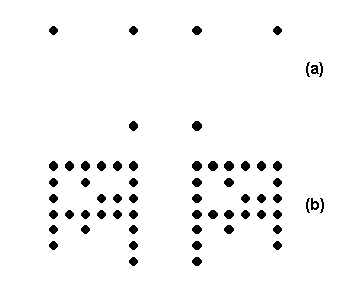
\includegraphics[scale = 1.10]{images/1.png}
	\caption{Рис. 1. Иллюстрация к понятию критических черт образа.}
	\label{image:1}
\end{figure}	



Обе пары картинок на Рис. 1 имеют общее свойство: в каждой из пар черная точка в правом нижнем углу заменена на белую, а белая точка левом нижнем углу - на черную. Такое изменение для нижней пары картинок (на рисунке - пара (b)), очевидно, является не более чем шумом, и оба образа (b) являются искаженными версиями одного и того же изображения. Тем самым, измененные точки не являются для этого образа критическими.

Совершенно иная ситуация имеет место для верхней пары картинок (a). Здесь такое же изменение точек оказывается слишком существенным для образа, так что правая и левая картинки являются различными образами. Следовательно, одна и та же черта образа может быть не существенной в одном случае, и критической в другом. Задачей нейронной сети будет формирование правильной реакции в обоих случаях: "пластичное" решение о появлении нового образа для пары (a) и "стабильное" решение о совпадении картинок (b). При этом выделение критической части информации должно получаться автоматически в процессе работы и обучения сети, на основе ее индивидуального опыта.

Отметим, что в общем случае одного лишь перечисления черт (даже если его предварительно выполнит человек, предполагая определенные условия дальнейшей работы сети) может оказаться недостаточно для успешного функционирования искусственной нейронной системы, критическими могут оказаться специфические связи между несколькими отдельными чертами.

Вторым значительным выводом теории выступает необходимость самоадатации алгоритма поиска образов в памяти. Нейронная сеть работает в постоянно изменяющихся условиях, так что предопределенная схема поиска, отвечающая некоторой структуре информации, может в дальнейшем оказаться неэффективной при изменении этой структуры. В теории адаптивного резонанса это достигается введением специализированной ориентирующей системы, которая самосогласованно прекращает дальнейший поиск резонанса в памяти, и принимает решение о новизне информации. Ориентирующая система также обучается в процессе работы.

В случае наличия резонанса теория АРТ предполагает возможность прямого доступа к образу памяти, откликнувшемуся на резонанс. В этом случает шаблон критических черт выступает ключем-прототипом для прямого доступа.

Эти и другие особенности теории адаптивного резонанса нашли свое отражение в нейросетевых архитектурах, которые получили такое же название - АРТ.

\section{Нейронная сеть AРT-1}
Имеется несколько разновидностей сетей АРТ. Исторически первой явилась сеть, в дальнейшем получившая название АРТ-1 (S.Grossberg, G.Carpenter, 1987). Эта сеть ориентирована на обработку образов, содержащих двоичную информацию. Дальнейший шаг - архитектура АРТ-2, опубликованная в том же 1987 году (S.Grossberg, G.Carpenter, 1987) - ориентирована на работу как с двоичными, так и с аналоговыми образами. В появившеемся относительно недавно сообщении о системе АРТ-3 (G.Carpenter, 1990) говорится о распространении адаптивной резонансной теории Гроссберга и Карпентер на многослойные нейроархитектуры. В нашей лекции мы остановимся на классической сети АРТ-1.

Нейросистема АРТ-1 является классификатором входных двоичных образов по нескольким сформированным сетью категориям. Решение принимается в виде возбуждения одного из нейронов распознающего слоя, в зависимости от степени похожести образа на шаблон критических черт данной категории. Если эта степень похожести невелика, т.е. образ не соответствует ни одной из имеющихся категорий, то для него формируется новый класс, который в дальнейшем будет модифицироваться и уточняться другими образами, формируя свой шаблон критических признаков. Для описания новой категории отводится новый, ранее не задействованный нейрон в слое распознавания.

Полное описание структуры сети адаптивного резонанса и теории ее работы, представленное в оригинальной публикации Гроссберга и Карпентер, является весьма громоздким, поэтому в своем изложении мы будем следовать более поздней книге Ф.Уоссермена , дополнив ее общим описанием особенностей АРТ-2 и новой архитектуры АРТ-3.

Сеть АРТ-1 состоит из пяти функциональных модулей (Рис. 11.2): двух слоев нейронов - слоя сравнения и слоя распознавания, и трех управляющих специализированных нейронов - сброса, управления 1 и управления 2.

\begin{figure}[h!]
	\centering
	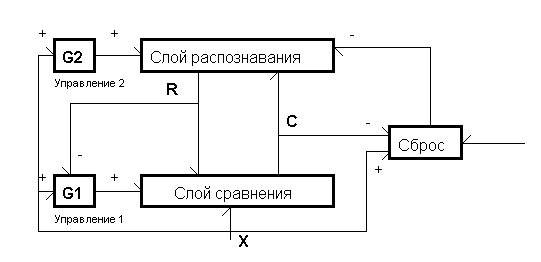
\includegraphics[scale = 1.10]{images/2.png}
	\caption{Рис. 2. Общая схема нейронной сети АРТ-1.}
	\label{image:1}
\end{figure}	



Начальное значение нейрона управления 1 полагается равным единице: G1=1. Входной двоичный вектор X поступает на слой сравнения, который первоначально пропускает его без изменения, при этом выходной вектор слоя сравнения C=X. Это достигается применением так называемого правила 2/3 для нейронов слоя сравнения. Каждый из нейронов этого слоя имеет три двоичных входа - сигнал от соответствующей компоненты вектора X, сигнал от нейрона управления 1 и сигнал обратной связи из слоя распознавания P (который в начальный момент равен нулю). Для активации нейрона в слое сравнения требуется, чтобы по крайней мере два из трех сигналов были равны единице, что и достигается в начальный момент входом от управления 1 и активными компонентами вектора X.

Выработанный слоем сравнения сигнал C поступает на входы нейронов слоя распознавания. Каждый нейрон слоя распознавания имеет вектор весов bj - действительных чисел, при этом возбуждается только один нейрон этого слоя, вектор весов которого наиболее близок к C. Это может быть достигнуто, например, за счет механизма латерального торможения типа "Победитель забирает все" (Лекция 7). Выход нейрона-победителя устанавливается равным единице, остальные нейроны полностью заторможены. Сигнал обратной связи от нейрона-победителя поступает обратно в слой сравнения через синаптические веса T. Вектор T, по существу, является носителем критических черт категории, определяемой выигравшим нейроном.

Выход нейрона управления 1 равен единице, только когда входной образ X имеет ненулевые компоненты, то есть этот нейрон выполняет функцию детекции факта поступления образа на вход. Однако, когда возникает ненулевой отклик нейронов слоя распознавания R, значение управления 1 зануляется G1=0.

Сигнал нейрона управления 2 также устанавливается на единицу при ненулевом векторе X. Задачей этого нейрона является погашение активность на слое распознавания, если в сеть не поступило никакой информации.

Итак, при генерации отклика R слоя распознавания выход G1=0, и теперь нейроны слоя сравнения активируются сигналами образа X и отклика R. Правило двух третей приводит к ативации только тех нейронов слоя сравнения, для которых и X, и R являются единичными. Таким образом, выход слоя сравнения C теперь уже не равен в точности X, а содержит лишь те компоненты X, которые соответствуют критическим чертам победившей категории. Этот механизм в теории АРТ получил название адаптивной фильтрации образа X.

Теперь задачей системы является установить, достаточен ли набор этих критических черт для окончательного отнесения образа X к категории нейрона-победителя. Эту функцию осуществляет нейрон сброса, который измеряет сходство между векторами X и C. выход нейрона сброса определяется отношением числа единичных компонент в векторе C к числу единичных компонент исходного образа X. Если это отношение ниже некоторого определенного уровня сходства, нейрон выдает сигнал сброса, означающий что уровень резонанса образа X с чертами предлагаемой категории не достаточен для положительного заключения о завершении классификации. Условием возникновения сигнала сброса является соотношение

,

где r < 1 - параметр сходства.

Сигнал сброса выполняет полное торможение нейрона-победителя-неудачника, который не принимает в дальнейшем участия в работе сети.

Опишем последовательно события, происходящие в сети АРТ в процессе классификации.

\subsection{Начальное состояние сети} 
Нулевые значения компонент входного вектора X устанавливают сигнал нейрона управления 2 в нуль, одновременно устанавливая в нуль выходы нейронов слоя распознавания. При возникновении ненулевых значений X, оба сигнала управления (G1 и G2) устанавливаются равными единице. При этом по правилу двух третей выходы нейронов слоя сравнения C в точности равны компонентам X.

Вектор C поступает на входы нейронов слоя распознавания, которые в конкурентной борьбе определяют нейрон-победитель, описывающий предполагаемый результат классификации. В итоге выходной вектор R слоя распознавания содержит ровно одну единичную компоненту, остальные значения равны нулю. Ненулевой выход нейрона-победителя устанавливает в нуль сигнал управления 1: G1=0. По обратной связи нейрон-победитель посылает сигналы в слой сравнения, и начинается фаза сравнения.

\subsection{Фаза сравнения}
В слое сравнения веер сигналов отклика слоя распознавания сравнивается с компонентами вектора X. Выход слоя сравнения C теперь содержит единичные компоненты только в тех позициях, в которых единицы имеются и у входного вектора X и у вектора обратной связи P. Если врезультате сравнения векторов C и X не будет обнаружено значительных отличий, то нейрон сброса остается неактивным. Вектор C вновь вызовет возбуждение того-же нейрона-победителя в слое распознавания, что и удачно завершит процесс классификации. В противном случае будет выработан сигнал сброса, который затормозит нейрон-победитель в слое распознавания, и начнется фаза поиска.

\subsection{Фаза поиска}
В результате действия тормозящего сигнала сброса все нейроны слоя распознавания получат нулевые выходы, и, следовательно, нейрон управления 1 примет единичное значение активности. Снова выходной сигнал слоя сравнения C установится равным в точности X, как и в начале работы сети. Однако теперь в конкурентной борьбе в слое распознавания предыдущий нейрон-победитель не участвует, и будет найдена новая категория - кандидат. После чего опять повторяется фаза сравнения.

Итерационный процесс поиска завершается двумя возможными способами.

Найдется запомненная категория, сходство которой с входным вектором X будет достаточным для успешной классификации. После этого происходит обучающий цикл, в котором модифицируются веса bi и ti векторов B и T возбужденного нейрона, осуществившего классификацию.
В процессе поиска все запомненные категории окажутся проверенными, но ни одна из них не дала требуемого сходства. В этом случае входной образ X об'является новым для нейросети, и ему выделяется новый нейрон в слое распознавания. Весовые вектора этого нейрона B и T устанавливаются равными вектору X.
Важно понимать, почему вообще требуется фаза поиска и окончательный результат классификации не возникает с первой попытки. Внимательный читатель вероятно уже обнаружил ответ на это вопрос. Обучение и функционирование сети АРТ происходит одновременно. Нейрон-победитель определяет в пространстве входных векторов ближайший к заданному входному образу вектор памяти, и если бы все черты исходного вектора были критическими, это и было бы верной классификацией. Однако множество критических черт стабилизируется лишь после относительно длительного обучения. На данной фазе обучения лишь некоторые компоненты входного вектора принадлежат актуальному множеству критических черт, поэтому может найтись другой нейрон-классификатор, который на множестве критических черт окажется ближе к исходному образу. Он и определяется в результате поиска.

Отметим, что после относительной стабилизации процесса обучения классификация выполняется без фазы поиска. В этом случае говорят, что формируется прямой доступ к памяти. Возникновение в процессе обучения прямого доступа доказывается в теории АРТ.

\subsection{Обучение сети АРТ}
В начале функционирования все веса B и T нейронов, а также параметр сходства получают начальные значения. Согласно теории АРТ, эти значения должны удовлетворять условию



где m - число компонент входного вектора X, значение L>1 (например L=2). Такой выбор весов будет приводить к устойчивому обучению. Уровень сходства r выбирается на основе требований решаемой задачи. При высоких значениях этого параметра будет сформировано большое число категорий, к каждой из которых будут относиться только очень похожие вектора. При низком уровне r сеть сформирует небольшое число категорий с высокой степенью обобщения.

Процесс обучения происходит без учителя, на основе самоорганизации. Обучение производится для весов нейрона-победителя в случае как успешной, так и неуспеншной классификации. При этом веса вектора B стремятся к нормализованной величине компонент вектора C:



При этом роль нормализации компонент крайне важна. Вектора с большим число единиц приводят к небольшим значениям весов b, и наоборот. Таким образом, произведение



оказывается масштабированным. Масштабирование приводит к тому, что возможно правильное различение векторов, даже если один является подмножеством другого. Пусть нейрон X1 соответствует образу (100000), а нейрон X2 - образу (111100). Эти образы являются, очевидно, различными. При обучении без нормализации (т.е. bi ® ci ) при поступлении в сеть первого образа, он даст одинаковые скалярные произведения, равные 1, как с весами нейрона X1, так и X2. Нейрон X2, в присутствии небольших шумовых отклонений в значениях весов, может выиграть конкуренцию. При этом веса его вектора T устаноятся равными (100000), и образ (111100) будет безвозвратно "забыт" сетью.
При применении нормализации исходные скалярные произведения будут равны единице для нейрона X1, и значению 2/5 для нейрона X2 (при L=2). Тем самым, нейрон X1 заслуженно и легко выиграет конкурентное соревнование.

Компоненты вектора T, как уже говорилось, при обучении устанавливаются равными соответвующим значениям вектора C. Следует подчеркнуть, что это процесс необратим. Если какая-то из компонент tj оказалась равной нулю, то при дальнейшем обучении на фазах сравнения соотвествующая компонента cj никогда не получит подкрепления от tj=0 по правилу 2/3, и, следовательно, единичное значение tj не может быть восстановлено. Обучение, таким образом, сопровождается занулением все большего числа компонент вектора T, оставшиеся ненулевыми компоненты определяют множество критических черт данной категории. Эта особенность проиллюстрирована на Рис. 3.

\begin{figure}[h!]
	\centering
	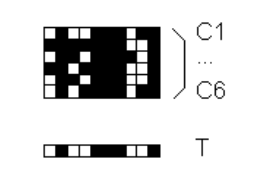
\includegraphics[scale = 1.10]{images/3.png}
	\caption{Рис. 3. Обучающие образы C и сформированный вектор критических черт T - минимальный набор общих элементов категории.}
	\label{image:1}
\end{figure}	


В оригинальной работе обучение рассматривается в терминах дифференциальных уравне-ний, из которых указанные нами значения получаются в виде предельных.

Остановимся теперь кратко на основных теоремах теории АРТ, характеризующих обучение и функционирование сети. Некоторые из них нами уже упоминались в тексте.

\section{Теоремы АРТ}
1. По достижении стабильного состояния обучения пред'явление одного из обучающих векторов будет сразу приводить к правильной классификации без фазы поиска, на основе прямого доступа.

2. Процесс поиска устойчив.

3. Процесс обучения устойчив. Обучение весов нейрона-победителя не приведет в дальнейшем к переключению на другой нейрон.

4. Процесс обучения конечен. Обученное состояние для заданного набора образов будет достигнуто за конечное число итерации, при этом дальнейшее пред'явление этих образов не вызовет циклических изменений значений весов.

\section{Дальнейшее развитие АРТ: архитектуры АРТ-2 и АРТ-3}
\subsection{Нерешенные проблемы и недостатки АРТ-1}
Нейронные сети АРТ, при всех их замечательных свойствах, имеют ряд недостатков. Одним из них является большое количество синаптических связей в сети, в расчете на единицу запоминаемой информации. При этом многие из весов этих связей (например, веткора T) оказываются после обучения нулевыми. Эту особенность следует учитывать при аппаратных реализациях.

Сеть АРТ-1 приспособлена к работе только с битовыми векторами. Это неудобство преодолевается в сетях АРТ-2 и АРТ-3. Однако в этих архитектурах, равно как и в АРТ-1, сохраняется главный недостаток АРТ - локализованность памяти. Память нейросети АРТ не является распределенной, некоторой заданной категории отвечает вполне конкретный нейрон слоя распознавания. При его разрушении теряется память обо всей категории. Эта особенность, увы, не позволяет говорить о сетях адаптивной резонансной теории, как о прямых моделях биологических нейронных сетей. Память последних является распределенной.

\subsection{Сети АРТ-2 и АРТ-3}
Основной отличительной чертой нейронной сети АРТ-2 является возможность работы с аналоговыми векторами и сигналами. По сравнению с АРТ-1 в архитектуре сети сделаны некоторые изменения, позволяющие отдельным подсистемам функционировать асинхронно, что принципиально для аппаратных реализаций.

Важным отличием аналоговых сигналов от битовых является принципиальная возможность аналоговых векторов быть сколь угодно близкими друг к другу (в то время как простанство битовых векторов дискретно). Это накладывает дополнительные требования на функционирование нейронов слоя сравнения - требуется более тонкий и чувствительный механизм для выделения областей резонанса. Общим решением здесь является переход к многослойной архитектуре, с все более точной настройкой при переходе от слоя к слою, что и применено в АРТ-2. Функционирование слоя распознавания принципиально не изменяется.

Сети АРТ-2 применялись для распознавания движущихся изображений. Успешные эксперименты выполнены в Массачусетском Технологическом Институте (MIT). Поскольку нейросистемы АРТ не содержат механизма инвариантного распознавания (в отличие от НЕОКОГНИТРОНА, см. предыдущую Лекцию), то в сочетании с ними применяются специализированные (часто не нейросетевые) системы инвариантного представления образов, например двумерное преобразование Фурье, или более сложные алгоритмы. Более подробное рассмотрение особенностей и применений АРТ-2 требует профессионального изучения и не входит в наши цели.

Следующим шагом в развитии АРТ явилась сеть АРТ-3. Особенности обучения нейронов сетей АРТ-1 и АРТ-2 не позволяют использовать эти сети, как элементы более крупных иерархических нейросистем, в частности, компоновать из них многослойные сети. Это затрудняет представление в АРТ иерархически организованной информации, что характерно для систем восприятия человека и животных.

Эти проблемы решены в сети АРТ-3, которая выступает как многослойная архитектура. При переходе от слоя к слою происходит контрастирование входных образов и запоминание их в виде все более общих категорий. При этом основной задачей каждого отдельного слоя является сжатие входящей информации.

Образ входит в адаптирующийся резонанс между некоторой парой слоев, в дальнейшем этот резонанс рапространяется на следующие слои иерархии. В АРТ-1 и АРТ-2 недостаточный уровень резонанса приводил к генерации сигнала сброса, что приводило к полному торможению слоя распознавания. В случае многослойной сети АРТ-3 это недопустимо, так как это разрывает поток информации. Поэтому в АРТ-3 введен специальный механизм зависимости активности синапсов обратных связей от времени, аналогичный рефрактерному торможению биологического нейрона после передачи возбуждения. Поэтому вместо полного сброса сигнала происходит торможение синаптических сигналов обратной связи, и слой сравнения получает исходное состояние возбуждения для выполнения фазы поиска нового резонанса.

Интересным предложением является также использование в многослойной иерархии слоев, которые не являются слоями АРТ, а принадлежат некоторой другой архитектуре. В этом случае система получается гибридной, что может привести к возникновению новых полезных свойств.

Развитие теории АРТ продолжается. По высказыванию авторов теории, АРТ представляет собой нечто существенно более конкретное, чем философское построение, но намного менее конкретное, чем законченная программа для компьютера. Однако уже в современном виде, опираясь на свою более чем 20-летнюю историю, сети АРТ демонстрируют свои успешные применения в различных областях. АРТ сделала также важный шаг в общей проблеме моделирования пластично-стабильного восприятия.




1) A.Gove, S.Grossberg, E.Mingolla, "Brightness perception, illusorycontours, and cortico-geniculate feedback", Visual Systems 
2) G.A.Carpenter, S.Grossberg, "Pattern Recognition by Self-Organizing Neural Networks", Cambribge, MA, MIT Press, 1991. 
3) G.A.Carpenter, S.Grossberg, "Normal and amnesia learning, recognition, and memory by a neural model of cortico- hippocampal interactions", 1993.


\end{document}